%
% $RCSfile: structured_and_procedural_programming.tex,v $
%
% Copyright (C) 2002-2008. Christian Heller.
%
% Permission is granted to copy, distribute and/or modify this document
% under the terms of the GNU Free Documentation License, Version 1.1 or
% any later version published by the Free Software Foundation; with no
% Invariant Sections, with no Front-Cover Texts and with no Back-Cover
% Texts. A copy of the license is included in the section entitled
% "GNU Free Documentation License".
%
% http://www.cybop.net
% - Cybernetics Oriented Programming -
%
% http://www.resmedicinae.org
% - Information in Medicine -
%
% Version: $Revision: 1.1 $ $Date: 2008-08-19 20:41:09 $ $Author: christian $
% Authors: Christian Heller <christian.heller@tuxtax.de>
%

\subsection{Structured- and Procedural Programming}
\label{structured_and_procedural_programming_heading}
\index{Structured- and Procedural Programming}
\index{SPP}
\index{Control Structure}
\index{Sequenced Step}
\index{Procedure}
\index{Subroutine}
\index{Wild Jump, Goto}
\index{Recursion}
\index{Hierarchical Modularisation of Control Structures}
\index{Entrance and Exit of a Control Structure}
\index{Module}
\index{Library}
\index{Program Flow Chart}
\index{Structure Chart}

Computer history has produced a whole plethora of high-level languages (an
overview is given in section \ref{language_history_heading}). They are to ease
the programming of applications which solve problems of an arbitrary domain.
Nearly all of them make use of a number of techniques that stem from the
so-called \emph{Structured- and Procedural Programming} (SPP).

These techniques arise from firstly the reduction of \emph{Control Structures} to a
minimal set of elements which can be combined arbitrarily in \emph{Sequenced Steps}.
Secondly, repeating algorithms can be defined as \emph{Procedure} and called as
subroutine. That way, wild \emph{Jumps} from one part of a program to another
are avoided. A procedure can also call itself which is known as \emph{Recursion}
\cite{philippow}.

It is possible to \emph{hierarchically modularise} all control structures, with
each structure having a defined \emph{Entrance} and \emph{Exit}. When
procedures are grouped together in a separate file, then this file is often
called \emph{Module} or \emph{Library}. Modules can contribute greatly to the
reuse and creation of clear program code.

Two kinds of diagrams are typically used to describe a (part of a) procedural
program semi-formally: \emph{Program Flow Chart} and \emph{Structure Chart}.
Both representations are based on sequences of control structures. The former
differs from the latter in the existence and appearance of certain graphical
elements; \emph{GoTo} instructions, for example, do not exist in structure
charts.

Following is a brief description of the most important control elements of SPP,
given in form of both, diagrams \cite{schiedermeier} and C program code
\cite{gcc}. These basic control techniques are: \emph{Assignment},
\emph{Branching} and \emph{Looping}.

%
% $RCSfile: assignment.tex,v $
%
% Copyright (C) 2002-2008. Christian Heller.
%
% Permission is granted to copy, distribute and/or modify this document
% under the terms of the GNU Free Documentation License, Version 1.1 or
% any later version published by the Free Software Foundation; with no
% Invariant Sections, with no Front-Cover Texts and with no Back-Cover
% Texts. A copy of the license is included in the section entitled
% "GNU Free Documentation License".
%
% http://www.cybop.net
% - Cybernetics Oriented Programming -
%
% http://www.resmedicinae.org
% - Information in Medicine -
%
% Version: $Revision: 1.1 $ $Date: 2008-08-19 20:41:05 $ $Author: christian $
% Authors: Christian Heller <christian.heller@tuxtax.de>
%

\subsubsection{Assignment}
\label{assignment_heading}
\index{Assignment}
\index{Statement}
\index{Operator}
\index{Operand}
\index{Expression}
\index{Operation}
\index{Variable}
\index{Data Value}
\index{Allocation}
\index{Declaration}
\index{Type}
\index{Identifier}
\index{Initial Value}
\index{Initialisation}
\index{Block}
\index{Compound Statement}
\index{Local Variable}

A \emph{Statement} (figure \ref{statement_figure}) is a sequence of operators
and operands \cite{cmanual}, to be evaluated (executed) by (the next lower
abstraction level of) a computer. It is also called an \emph{Expression}. The
\emph{Operator} represents the actual \emph{Operation}, an active instruction
to the computer. It uses and works on passive data -- the \emph{Operands}, also
called \emph{Variables}. Following a statement in \emph{C} code:

\begin{scriptsize}
    \begin{verbatim}
    operand++;
    \end{verbatim}
\end{scriptsize}

\begin{figure}[ht]
    \begin{center}
        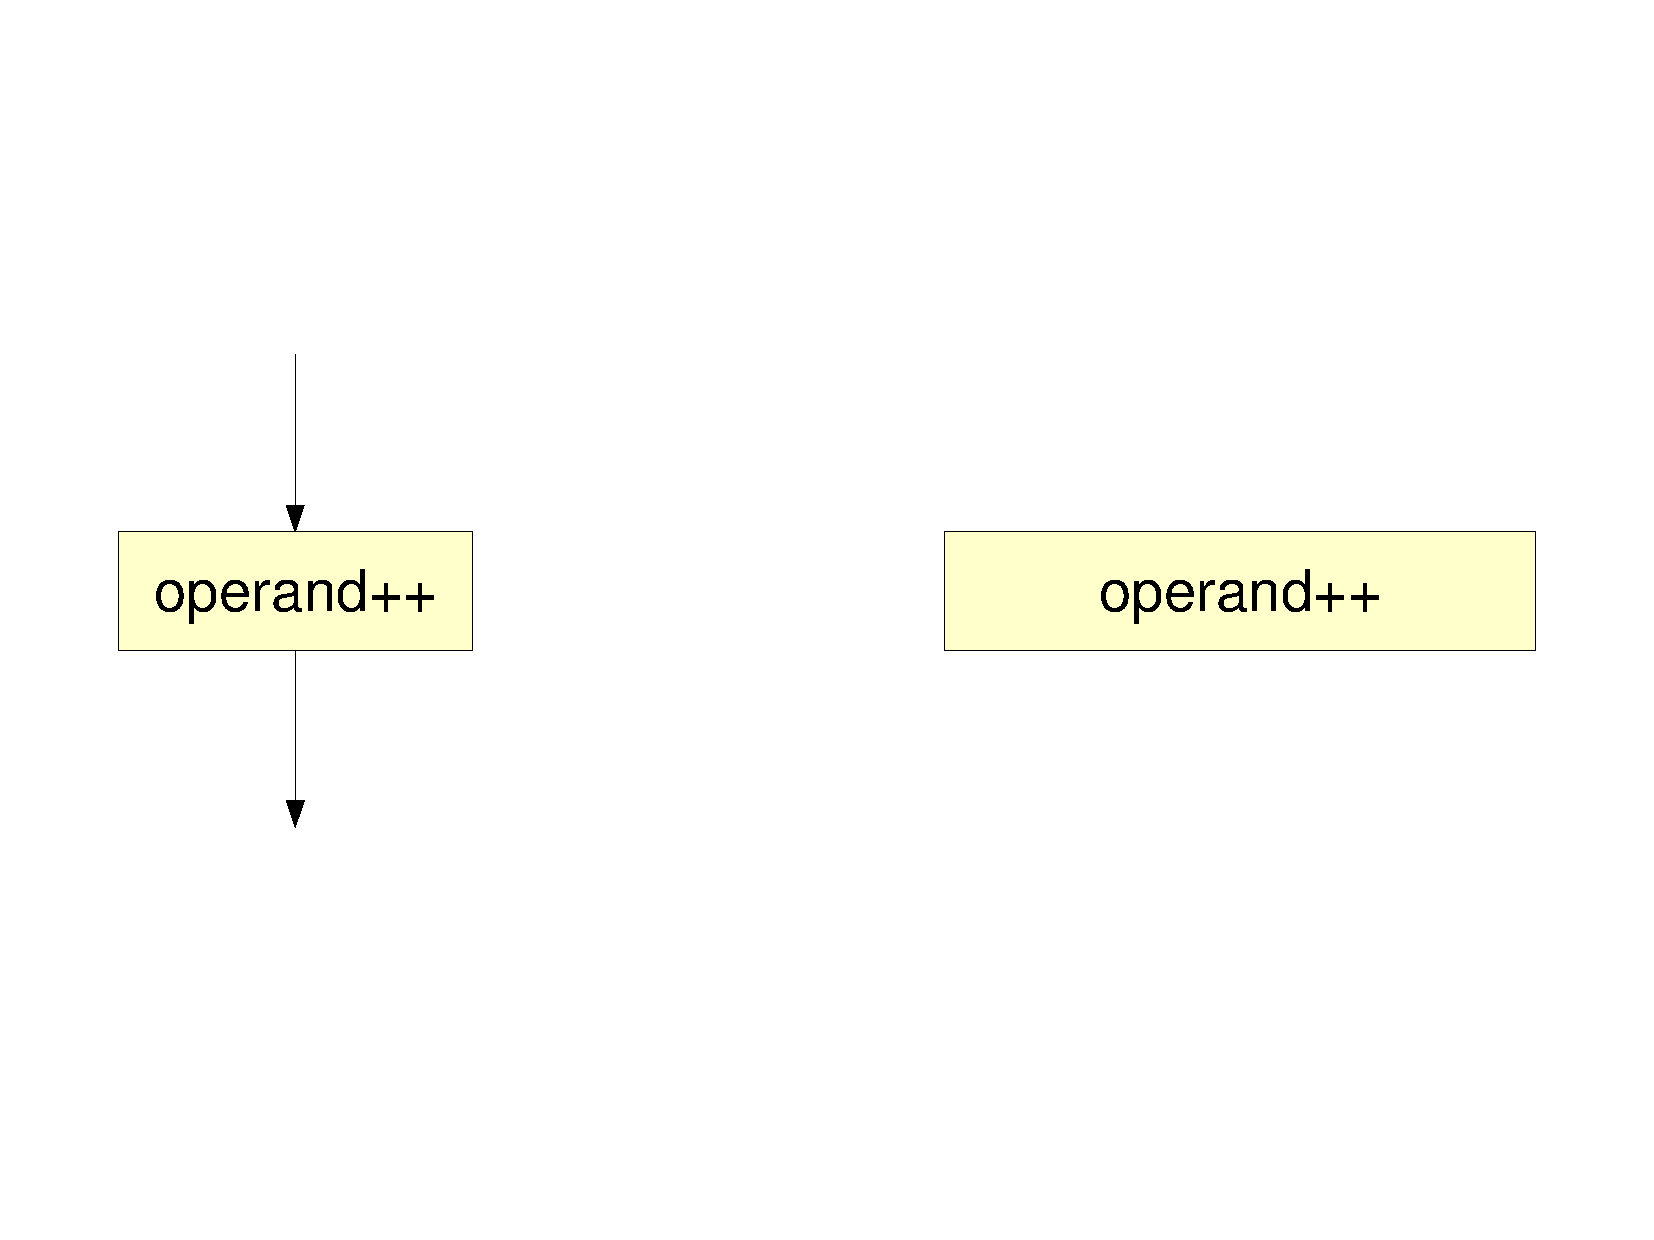
\includegraphics[scale=0.3,angle=-90]{graphic/statement.pdf}
        \caption{Statement as Program Flow Chart and Structure Chart}
        \label{statement_figure}
    \end{center}
\end{figure}

A \emph{Variable} is a placeholder for an abstracted \emph{Data Value}. It
occupies space in memory which is why this space has to be reserved before it
can be used. The reservation is called \emph{Allocation} or \emph{Declaration}
and it states the variable's \emph{Type} and an \emph{Identifier}. Commonly,
variables also get initialised through the \emph{Assignment} of an
\emph{Initial Value}. Here an example for declaration and initialisation
through assignment in \emph{C} code:

\begin{scriptsize}
    \begin{verbatim}
    type identifier = value;
    \end{verbatim}
\end{scriptsize}

Many statements which belong together can form a \emph{Block}, also called
\emph{Compound Statement}. Variables declared in a block are called its
\emph{Local Variables} and loose their validity outside that block. Blocks have
an opening and a closing symbol. Following once more an example in \emph{C}
programming language source code, showing a block with two statements:

\begin{scriptsize}
    \begin{verbatim}
    {
        statement1;
        statement2;
    }
    \end{verbatim}
\end{scriptsize}

%
% $RCSfile: branching.tex,v $
%
% Copyright (C) 2002-2008. Christian Heller.
%
% Permission is granted to copy, distribute and/or modify this document
% under the terms of the GNU Free Documentation License, Version 1.1 or
% any later version published by the Free Software Foundation; with no
% Invariant Sections, with no Front-Cover Texts and with no Back-Cover
% Texts. A copy of the license is included in the section entitled
% "GNU Free Documentation License".
%
% http://www.cybop.net
% - Cybernetics Oriented Programming -
%
% http://www.resmedicinae.org
% - Information in Medicine -
%
% Version: $Revision: 1.1 $ $Date: 2008-08-19 20:41:05 $ $Author: christian $
% Authors: Christian Heller <christian.heller@tuxtax.de>
%

\subsubsection{Branching}
\label{branching_heading}
\index{Branching}
\index{Branch}
\index{Conditional Branching}
\index{Unconditional Branching}
\index{Goto (Jump) Command}
\index{Condition}
\index{Alternative}
\index{Choice}
\index{Multiple Condition}
\index{Switch}
\index{Case}

A block of statements that get only executed at special occasions is called a
\emph{Branch}. Two kinds of branching exist: \emph{Conditional Branching} and
\emph{Unconditional Branching}. An implementation of the latter is the well-known
but also disliked \emph{goto} (\emph{jump}) command. The former depends on a
\emph{Condition}, also called \emph{Alternative} or \emph{Choice} (figure
\ref{condition_figure}), that is its statements are only executed if the
condition's result is true. That way, a condition can change the flow of a
program. A code example follows; it shows conditional branching:

\begin{scriptsize}
    \begin{verbatim}
    if (condition) {
        statements;
    } else {
        statements;
    }
    \end{verbatim}
\end{scriptsize}

\begin{figure}[ht]
    \begin{center}
        \includegraphics[scale=0.3,angle=-90]{graphic/condition.pdf}
        \caption{Condition as Program Flow Chart and Structure Chart}
        \label{condition_figure}
    \end{center}
\end{figure}

Many programming languages offer a \emph{Multiple Condition} control structure
like \emph{switch} or \emph{case}. It is a comfortable possibility to let a
program make a choice out of many alternatives:

\begin{scriptsize}
    \begin{verbatim}
    switch (condition) {
        case constant1:
            statements;
        case constant2:
            statements;
        default:
            statements;
    }
    \end{verbatim}
\end{scriptsize}

Essentially, however, it is a subsumption of a number of simple conditions which
are mostly called \emph{if-else}, and therefore replaceable by such, as shown
following:

\begin{scriptsize}
    \begin{verbatim}
    if (condition == constant1) {
        statements;
    } else if (condition == constant2) {
        statements;
    } else {
        statements;
    }
    \end{verbatim}
\end{scriptsize}

The multiple condition is conceptually no innovation in comparison with the
simple condition and hence pure convenience for the programmer. The interpreter
described in chapter \ref{cybernetics_oriented_interpreter_heading} uses solely
if-then statements.

%
% $RCSfile: looping.tex,v $
%
% Copyright (C) 2002-2008. Christian Heller.
%
% Permission is granted to copy, distribute and/or modify this document
% under the terms of the GNU Free Documentation License, Version 1.1 or
% any later version published by the Free Software Foundation; with no
% Invariant Sections, with no Front-Cover Texts and with no Back-Cover
% Texts. A copy of the license is included in the section entitled
% "GNU Free Documentation License".
%
% http://www.cybop.net
% - Cybernetics Oriented Programming -
%
% http://www.resmedicinae.org
% - Information in Medicine -
%
% Version: $Revision: 1.1 $ $Date: 2008-08-19 20:41:07 $ $Author: christian $
% Authors: Christian Heller <christian.heller@tuxtax.de>
%

\subsubsection{Looping}
\label{looping_heading}
\index{Looping}
\index{Loop Control Structure}
\index{Pre Test Loop}
\index{Post Test Loop}
\index{Counting Loop}
\index{while, while-do}
\index{do-while, repeat-until}
\index{for, for-next}

The \emph{Loop} (figure \ref{loop_figure}) is a control element that allows to
iterate through statements, in other words to execute them repeatedly, several
times. Its concept is quite simple -- a jump backwards in the program. However,
this low-level jump is hidden to the application programmer using a higher-level
SPP language. The loop is indicated by a special keyword instead, for example:

\begin{scriptsize}
    \begin{verbatim}
    while (condition) {
        statements;
    }
    \end{verbatim}
\end{scriptsize}

\begin{figure}[ht]
    \begin{center}
        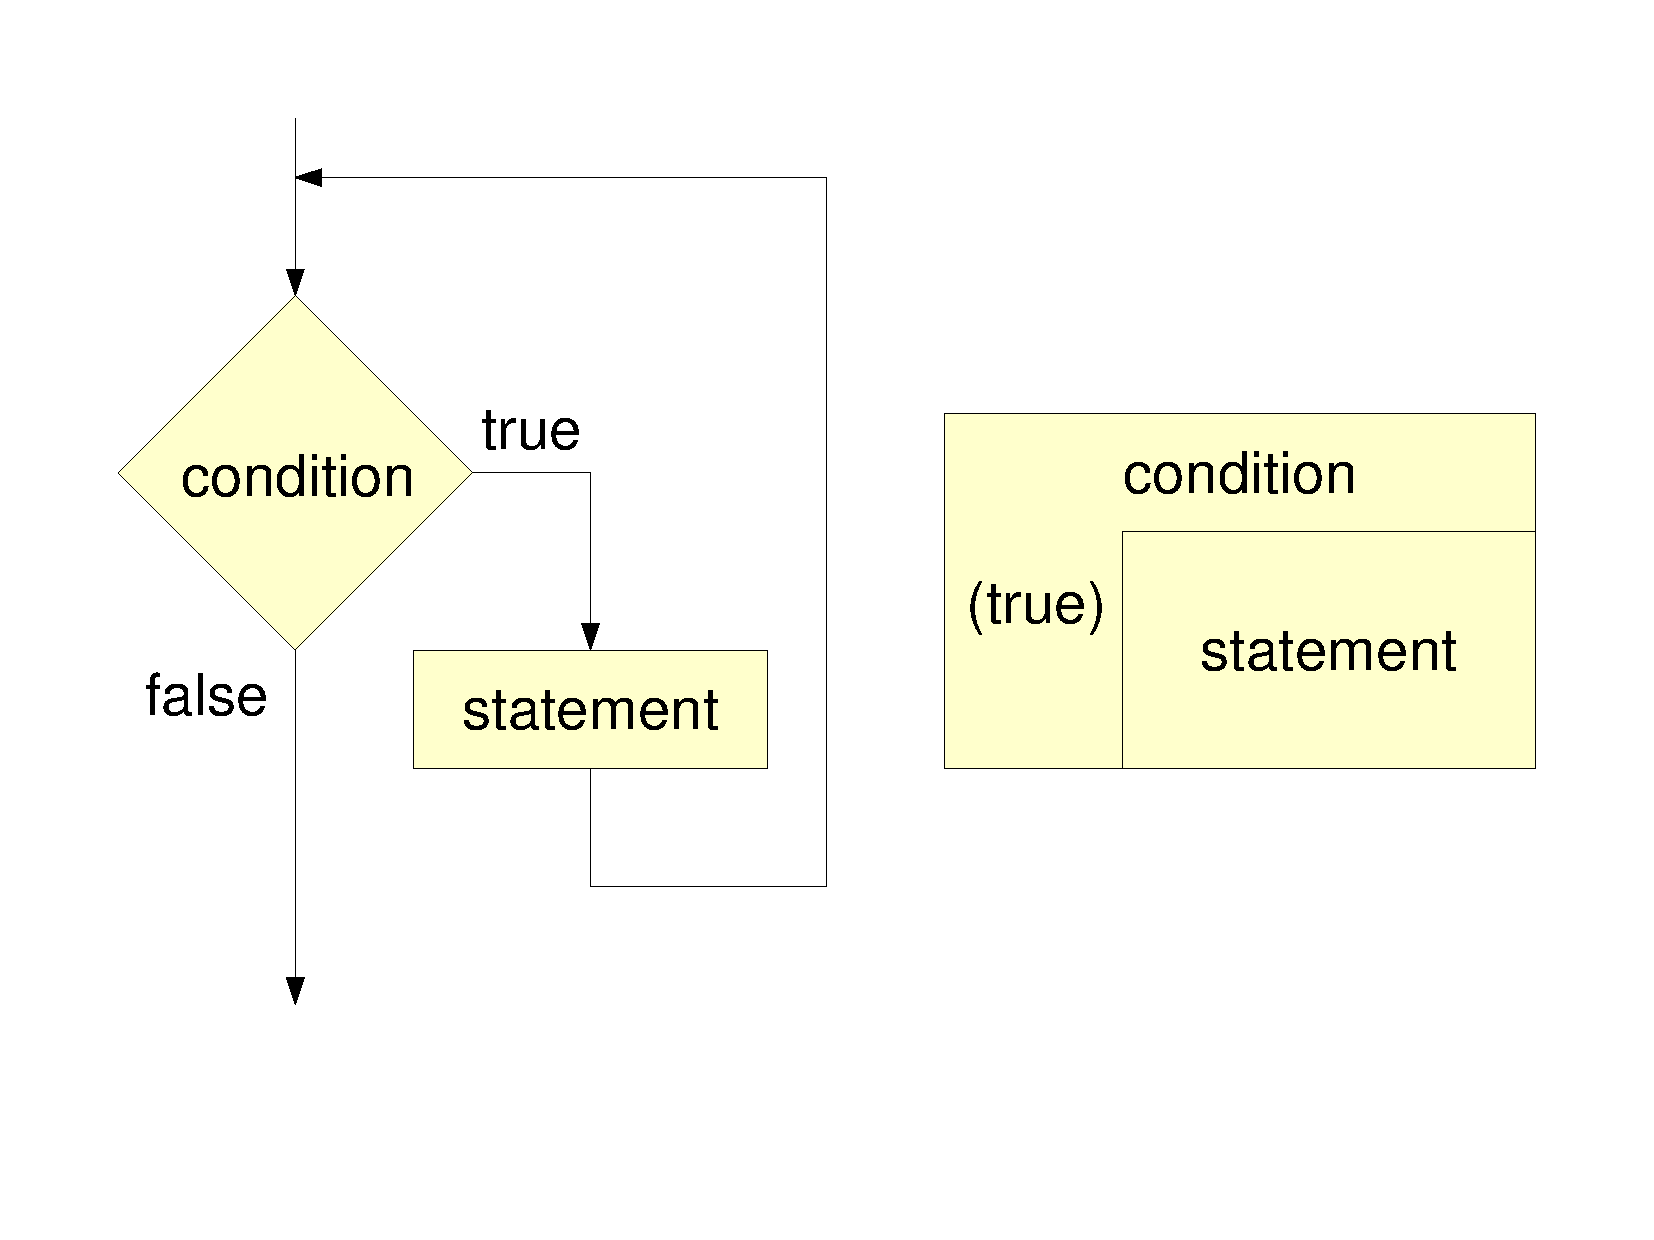
\includegraphics[scale=0.3,angle=-90]{graphic/loop.pdf}
        \caption{Loop as Program Flow Chart and Structure Chart}
        \label{loop_figure}
    \end{center}
\end{figure}

Most programming languages offer three different loop styles, as there are:

\begin{itemize}
    \item[-] Pre-test loop: \emph{while}, \emph{while-do}
    \item[-] Post-test loop: \emph{do-while}, \emph{repeat-until}
    \item[-] Counting Loop: \emph{for}, \emph{for-next}
\end{itemize}

A \emph{Pre-Test Loop} is used when one wants to check a condition before the
statements in the loop body are executed:

\begin{scriptsize}
    \begin{verbatim}
    int i = 0;
    while (i < 1) {
        statements;
        i++;
    }
    \end{verbatim}
\end{scriptsize}

The \emph{Post-Test Loop}, on the other hand, repeats all loop-body statements
until a condition is met:

\begin{scriptsize}
    \begin{verbatim}
    int i = 0;
    do {
        statements;
        i++;
    } while (i < 1);
    \end{verbatim}
\end{scriptsize}

A \emph{Counting Loop}, finally, can be applied when the number of necessary
repetitions of the loop-body statements is known in advance:

\begin{scriptsize}
    \begin{verbatim}
    int i;
    for (i = 0; i < 1; i++) {
        statements;
    }
    \end{verbatim}
\end{scriptsize}

The statements in all three loop examples are only executed once. It is not
difficult to see that the \emph{for} loop can be replaced with a \emph{while}
loop by initialising the \emph{i} variable in its declaration line and moving
the increment statement into the loop's block. But also the \emph{do-while}
loop can be replaced with a \emph{while} loop. If the behaviour does not match
(for example a while block is not executed even once), then changing the initial
loop variable value can solve this problem. Otherwise, modifying the statements
(algorithm) in the block, without changing it logically, will do.

As can be seen: Most variations of the \emph{Looping} concept are just a
convenience for the programmer. They are conceptually identical and can be lead
back to a simple loop with break condition, each. The interpreter described in
chapter \ref{cybernetics_oriented_interpreter_heading} uses just one kind of
loop.

